\documentclass{article}


\usepackage[letterpaper, margin=1.3in]{geometry}
\usepackage[version=3]{mhchem} % Formula subscripts using \ce{}
\usepackage[T1]{fontenc}       % Use modern font encodings
\usepackage{multirow}
\usepackage{subcaption}
\usepackage{booktabs}
\usepackage{fancyhdr}

\pagestyle{fancy}
\fancyhf{}
\lhead{Supoprting Information}
\fancyfoot[C]{S--\thepage}
\begin{document}	

{\Huge Enhanced Global PTM Discovery (G-PTM-D) with MetaMorpheus}

{\Large Stefan K. Solntsev\textsuperscript{1}, Michael R. Shortreed\textsuperscript{1}, Brian L. Frey\textsuperscript{1}, Lloyd M. Smith\textsuperscript{1,2}}\\
{\footnotesize 1 Department of Chemistry, University of Wisconsin-Madison, Madison, WI, USA}\\
{\footnotesize 2 Genome Center of Wisconsin, University of Wisconsin-Madison, Madison, WI, USA}\\

\section{Table of Contents}


\begin{enumerate}
\item \textbf{Table S1} The complete list of modifications used for enhanced G-PTM-D\\
      See Excel file
\item \textbf{Document S1}   A brief description of the calibration methodology      \hfill      Page S-1
\end{enumerate}

\newpage

{\huge \textbf{Document S1:} A brief description of the calibration methodology}

The calibration procedure is motivated by the software lock mass concept recently reported by the Mann group. 
In MetaMorpheus it is comprised of a nested cycle of a database searches, data point acquisition procedures, calibration curve fitting, and peak alignment procedures. 

\begin{figure}[ht]
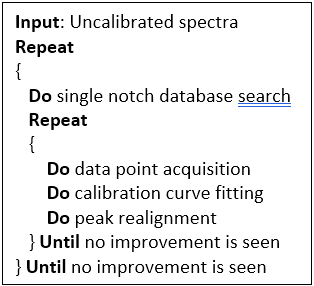
\includegraphics{supFig1.png}
\end{figure}

The narrow-window database search is run with precursor and parent mass tolerances that are appropriate for the uncalibrated spectra file. The target PSMs within 1\% false discovery rate are good identifications to be used in the data point acquisition step. 

The data point acquisition considers every identification in the confident PSMs, and searches the corresponding fragmentation spectra for peaks matching the fragments, considering different charge states and isotopic peaks for each fragment. If there is ambiguity as to which peak match a certain fragment, the corresponding match is discarded, because of the desire to use the most confident peaks for calibration, and an abundance of unambiguous peaks. If a sufficient number of such peaks is found, the identification is confident enough for calibration. Peaks corresponding to the unfragmented peptide in neighboring MS spectra are then gathered. Every accepted peak is a data point for the subsequent calibration curve fitting: every data point is comprised of the following numerical values:

\begin{itemize}
\item \textbf{Features:} m/z value,Retention time,Total ion count,Injection time
\item \textbf{Label:} m/z error
\end{itemize}

The inputs are the values that are available for every peak in the uncalibrated spectra, and would be used as inputs to the chosen calibration function. In addition to those, the confident identification, by means of a theoretical isotopic distribution, provides a Label for each data point, which is the difference between the observed and the expected m/z value of the peak. The calibration procedure relies on the assumption that peaks with similar inputs would have similar labels in the m/z value of the error.

Once the peaks are gathered, the data point set is split into a training and testing sets, where the training set is used to create several calibration curves, and a testing set is used to select the best curve based on the Mean Squared Error.

The contribution of every input variable to the error is modeled either as a linear function (chosen for simplicity and to account for instrument miscalibration) or as a random forest. The random forest model allows for non-linear relationship between an input variable and the m/z error, such as random ambient time-resolved fluctuations. The trained model is used to calibrate all the peaks in the spectra, by shifting the m/z value of the peak by an appropriate amount.

This procedure is repeated on a single collection of data points, and on multiple rounds of database searching. 

If a well-calibrated file is given as an input, no changes are made. This is because the calibration procedure only accepts changes if a test database search results in improvement.

Resulting calibrated spectra are written to an mzML file that may be used in subsequent MetaMorpheus tasks, or in any external software that may benefit from increased mass accuracy in the spectra.

\newpage

{\huge \textbf{Document S2:} }

\end{document}
